\documentclass[border=2mm]{standalone}
\usepackage{charter}
\usepackage{tikz}
\usepackage{xcolor}
\definecolor{blue}{RGB}{0, 114, 178}
\definecolor{red}{RGB}{213, 94, 0}

\begin{document}
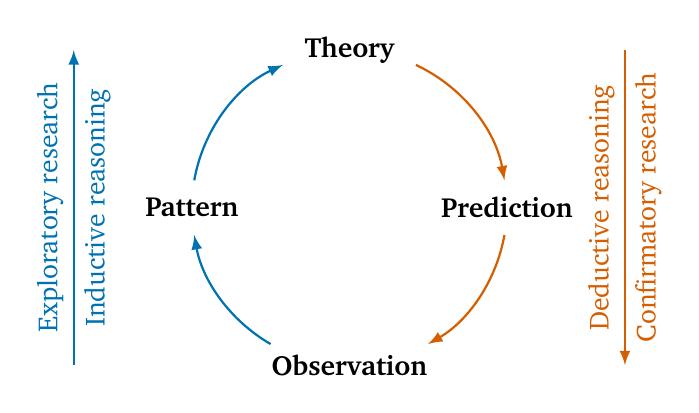
\begin{tikzpicture}
\foreach \a/\t in {90/Theory, 0/Prediction, -90/Observation, -180/Pattern}{
    \node (\t) at (\a:2cm) {\textbf{\t}};
}

% Circle lines
\draw[-latex, thick, red] (90-25:2cm) arc (90-25:0+10:2cm);
\draw[-latex, thick, red] (0-10:2cm) arc (0-10:-90+30:2cm);
\draw[-latex, thick, blue] (-90-30:2cm) arc (-90-30:-180+10:2cm);
\draw[-latex, thick, blue] (-180-10:2cm) arc (-180-10:-270+25:2cm);

% Exploratory
\draw[latex-, thick, blue] (-3.5,2) -- (-3.5,-2) node[blue, midway, anchor=north, rotate=90] {Inductive reasoning} node[blue, midway, anchor=south, rotate=90] {Exploratory research};

% Deductive
\draw[-latex, thick, red] (3.5,2) -- (3.5,-2) node[red, midway, anchor=south, rotate=90] {Deductive reasoning} node[red, midway, anchor=north, rotate=90] {Confirmatory research};

\end{tikzpicture}
\end{document}